\documentclass[crop,tikz]{standalone}

\usepackage{amsmath}
\usepackage{pgfplots}
\tikzset{>=latex}

\pgfplotsset{
  every non boxed x axis/.append style={
    axis line style={-latex}
  },
  every non boxed y axis/.append style={
    axis line style={-latex}
  },
  inverted/.style = {
    every axis legend/.append style={
      draw=white,
      fill=black,
      text=white
    }
  }
}

\begin{document}
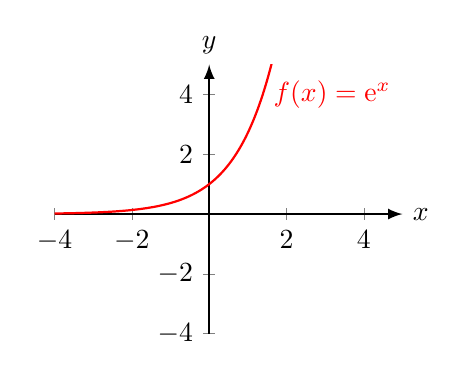
\begin{tikzpicture}
\begin{axis}[
  thick,
  width=6cm,
  height=5cm,
  domain=-4:2,
  samples=50,
  axis y line=middle,
  axis x line=middle,
  xlabel={$x$},
  ylabel={$y$},
  xlabel style={right},
  ylabel style={above},
  xmin=-4, xmax=5,
  ymin=-4, ymax=5
  ]
  \addplot[red,smooth] { exp(x) };
  \node[red,right] at (axis cs:1.4,4) {$f(x)=\operatorname{e}^x$};
\end{axis}
\end{tikzpicture}
\end{document}
